\documentclass{article}
\usepackage{tcolorbox}
\usepackage{xcolor}
\usepackage{graphicx}
\newcommand\crule[3][black]{\textcolor{#1}{\rule{#2}{#3}}}
\graphicspath{{./Analysis/Images/}}
\usepackage{subfiles}
\usepackage[english]{babel}
\usepackage{todonotes}
\usepackage{hyperref}
\hypersetup{
    colorlinks=true,
    urlcolor=magenta
    }
\usepackage{siunitx}
\usepackage{float}    
\usepackage{booktabs}
\usepackage[top=2cm,left=2cm,bottom=2cm,right=2cm]{geometry}
\usepackage{times}
\usepackage{multicol, caption}

\usepackage{titlesec} % required package for \titleformat
\titleformat*{\subsection}{\normalsize\bfseries} % size and style of the subsections
\usepackage[font=footnotesize,labelfont=bf]{caption} % size and style of the captions

\raggedcolumns
%\bibliography{References}
\usepackage{csquotes}
\usepackage[backend=biber,style=numeric,sorting=none]{biblatex}
\addbibresource{References.bib}

\definecolor{light-orange}{cmyk}{0,0.06,0.12,0.02}
\title{Observations of bloom dynamics in the Bornholm Basin from gliders}
\author{Jonas Dietrich, Alma Holmsten, Augusta Olsson, Marie Wicklander, Julia Mari Murata}
\date{\today}

\begin{document}
\maketitle


\subfile{Sections/Abstract}
\begin{multicols}{2}
\subfile{Sections/Introduction}
\subfile{Sections/MaterialsAndMethods}
\subfile{Sections/Result}
\end{multicols}

\begin{figure}[H]
  \centering
    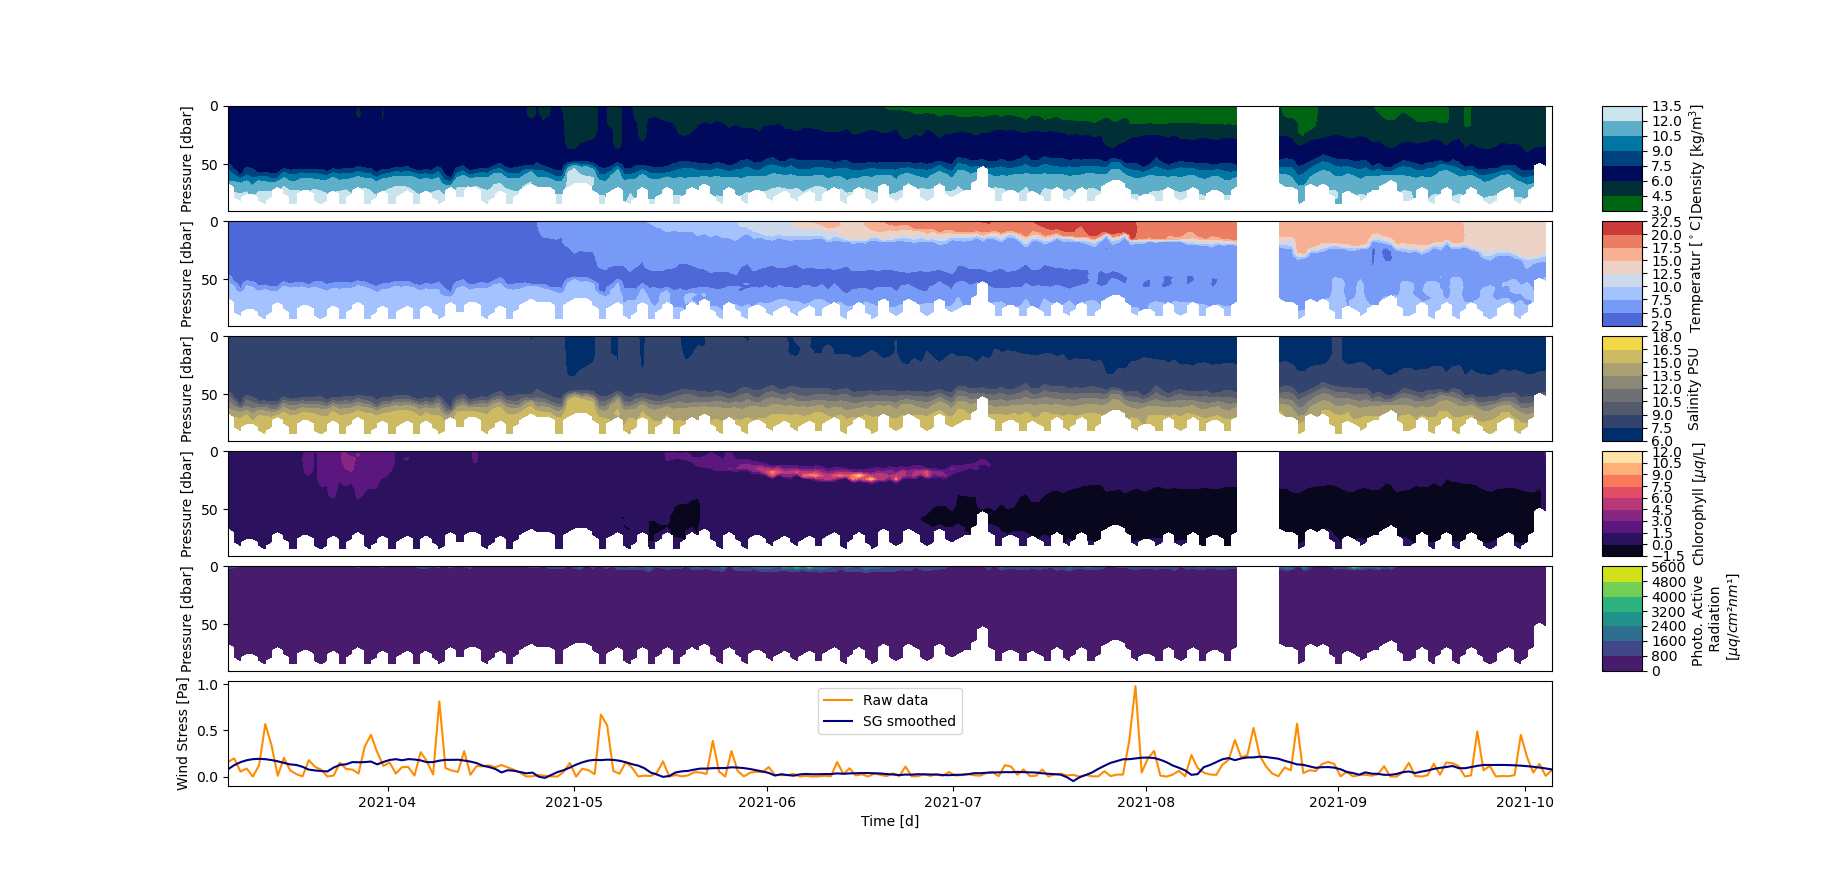
\includegraphics[width=\textwidth]{All_Properties.png}
\caption{Figures A-F show the change in physical parameters over time from the surface water layer to about \SI{80}{m} depth in the balitc. 
Shown are the six different physical parameters density (A), temperature (B),
salinity (C), chlorophyll (D), photosynthetically active radiation (E), and wind stress (F). For easy evaluation of wind stress, a Savitzky-Golay filter was used with a window size of 21 and a polynomial order of 3.}
  \label{fig:all}
\end{figure}

\begin{multicols}{2}
\subfile{Sections/Discussion}
\subfile{Sections/Conclusion}
\printbibliography
\end{multicols}


%\subfile{Sections/Appendix}

\end{document}
